%!TEX program = xelatex 
% where <program> is any of pdflatex, xelatex or lualatex
%% 

% install theme : https://github.com/matze/mtheme
% intall fonts : http://www.carrois.com/fira-4-1/ 

\documentclass[10pt]{beamer}

\usetheme{metropolis}

\usepackage{grffile}

\usepackage{booktabs}
\usepackage[scale=2]{ccicons}

\usepackage{pgfplots}
\usepgfplotslibrary{dateplot}

\usepackage{xspace}
\newcommand{\themename}{\textbf{\textsc{metropolis}}\xspace}
\setbeamertemplate{bibliography item}{\insertbiblabel}

\title{Characterizing earthquakes source physics with source scanning algorithms.}
\subtitle{A better earthquake analysis}
\author{Frederick Massin\inst{1} \& Alison Malcolm\inst{2}}
\institute{\inst{1} Post-doc \& \inst{2} Prof. \& Chevron Chair in Reservoir Characterization, Earth Sciences Department, MUN.}
\date{\today}
\titlegraphic{\hfill\includegraphics[height=1.0cm]{../material/logo}}

\begin{document}

\maketitle

\begin{frame}{Outline}
  \setbeamertemplate{section in toc}[sections numbered]
  \tableofcontents[hideallsubsections]
\end{frame}

\section{Shift \& stack approaches}

\begin{frame}{Why?}

	\begin{itemize} [<+- | alert@+>]
    \item Quantify the earthquakes physical properties \& uncertainties from continuous signals.
    \begin{itemize} [<+- | alert@+>]
      \item Probabilistic earthquake nucleation understanding and hazard assessment.
      \begin{itemize} [<+- | alert@+>]
        \item Earthquakes could be triggered by local stress perturbation from many sources, natural or not, with implications for the rupture characteristics.
        \end{itemize} \end{itemize} \end{itemize}    
    \only<3>{
      \begin{figure}  
        \includegraphics[height=0.45\textheight]{/Users/massin/Documents/Presentations/201511_postdoc-mun/2016-02-22_GAC-NL/material/FigA9-Upward_YLES.pdf}
        \caption{The 2008-9 Yellowstone Lake eq. swarm.}\label{yles}
      \end{figure} }
      
\end{frame}

\begin{frame}{Conventional approach}
	\begin{itemize}
		\item Arrival times (data reduced to minimum) => Hypocenter
		\only<2->{\item Long period signals (filtered data) => Moment tensor}
		\only<3->{\item Modeling of:
		\begin{itemize}
      \item slip distribution,
			\item stresses perturbation,
			\item ground deformation.
		\end{itemize}}
	\end{itemize}

  \only<1>{
    \begin{figure}  
      \includegraphics[height=0.5\textheight]{/Users/massin/Documents/Presentations/201511_postdoc-mun/2016-02-22_GAC-NL/material/matchfilt.png}
      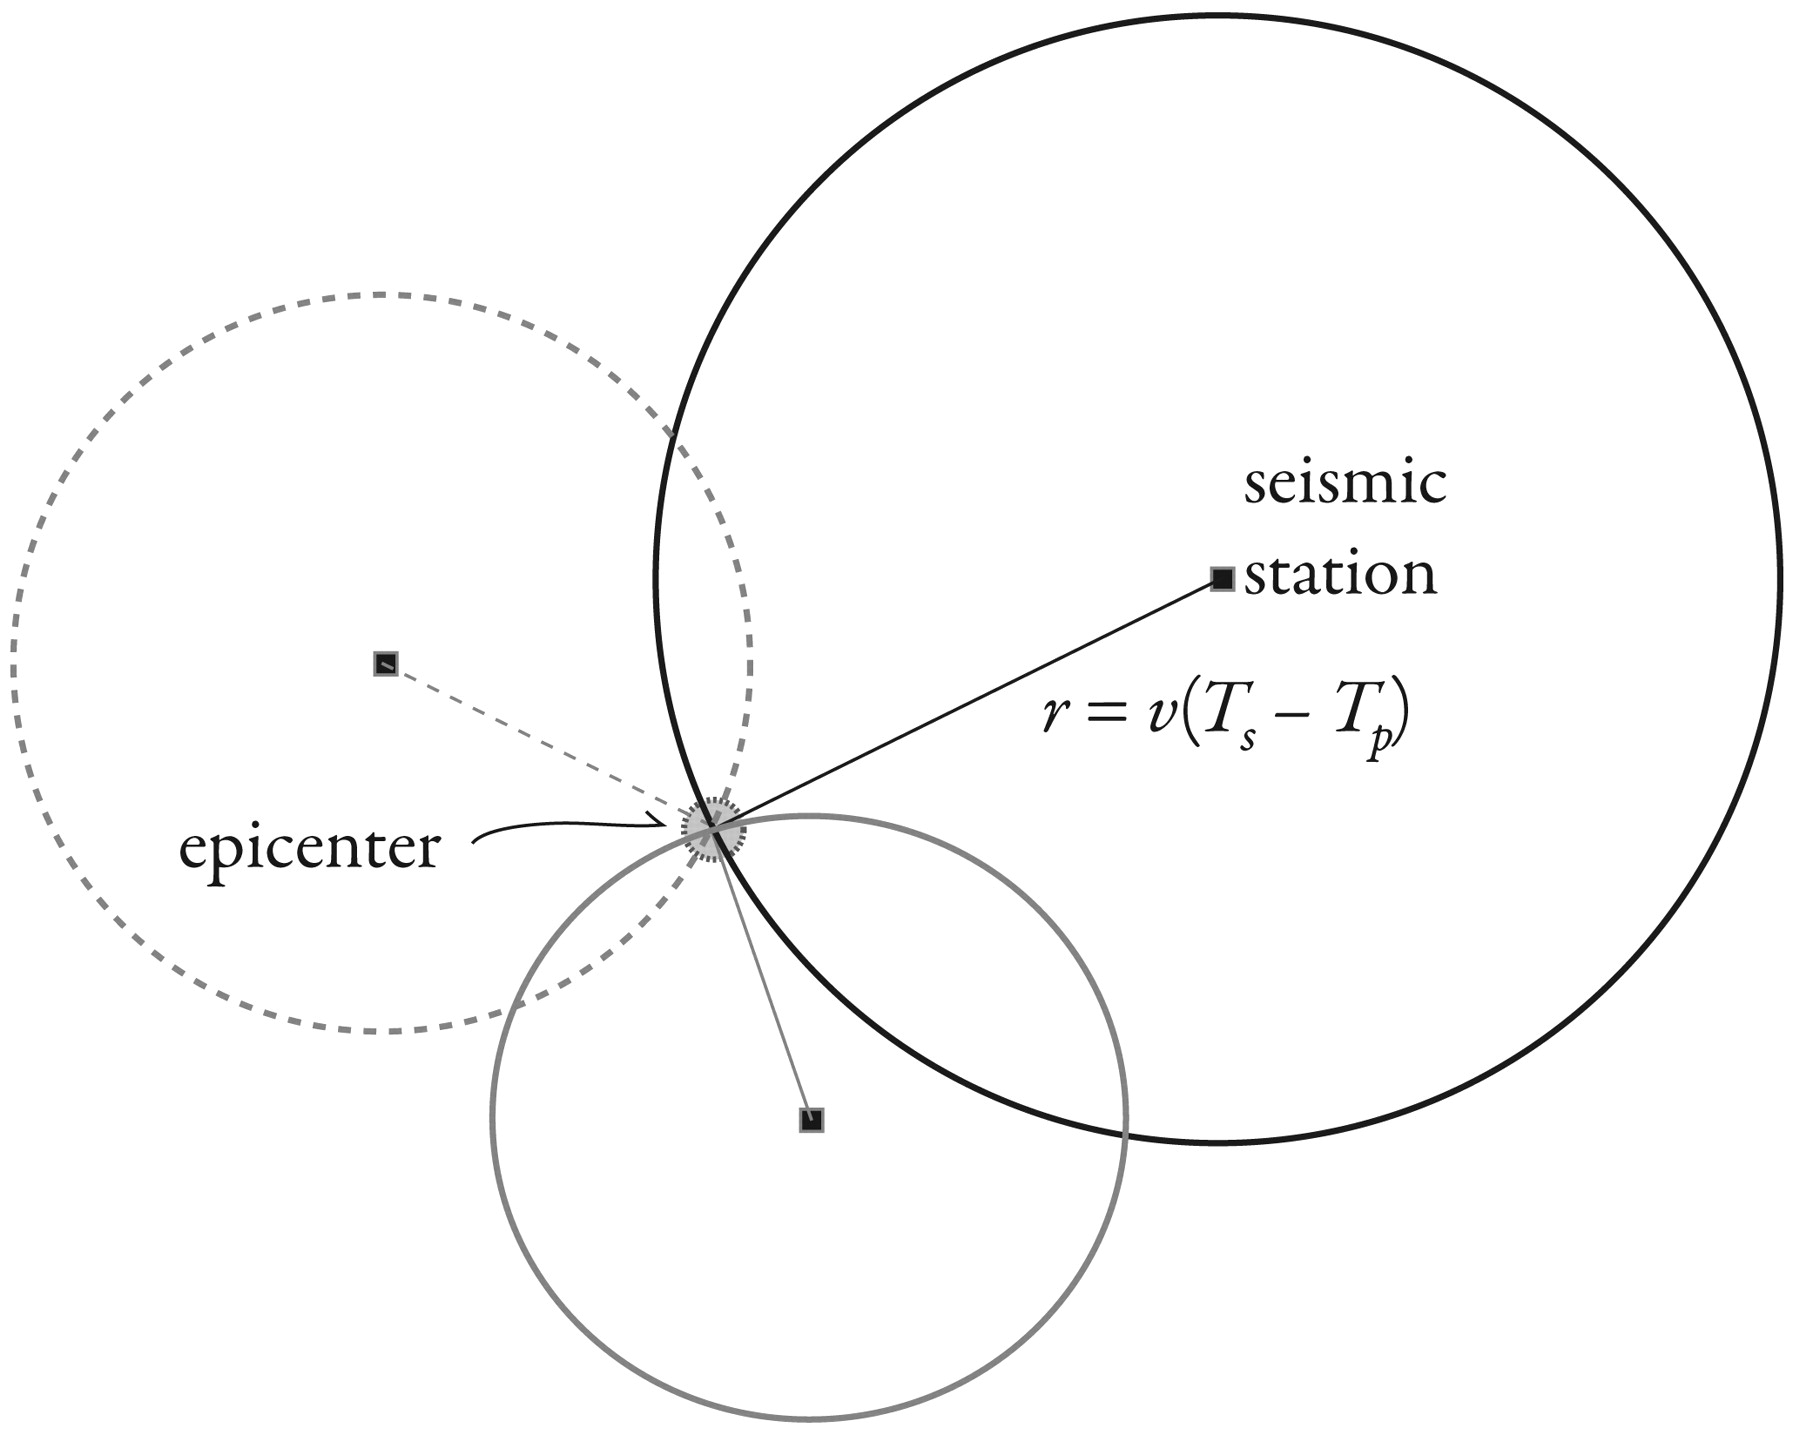
\includegraphics[height=0.5\textheight]{/Users/massin/Google Drive/Documents/Projects/MUN/slideshows/2016-02-14_group-meeting/materials/F1.large.jpg}
      \caption{From picks to precise location \cite{Waldhauser:2000ur}.}\label{picklocreloc}
    \end{figure} }
  

  \only<2>{
    \begin{figure}  
      % \includegraphics[height=0.5\textheight]{/Users/massin/Documents/Presentations/201511_postdoc-mun/2016-02-22_GAC-NL/material/spectmo.pdf}
      \includegraphics[height=0.5\textheight]{/Users/massin/Documents/Presentations/201511_postdoc-mun/2016-02-22_GAC-NL/material/full-Mo.png} 
      \caption{... to moment tensor \cite{Godano:2015ti}.}\label{mo}
    \end{figure} }

    \only<3>{
    \begin{figure}  
      \includegraphics[height=0.4\textheight]{/Users/massin/Documents/Presentations/201511_postdoc-mun/2016-02-22_GAC-NL/material/stresschange.pdf}
      \caption{... to stress change.}\label{stress}
    \end{figure} }

	\only<4>{\textbf{\textit{How to use more data in source parameters analysis ? In a more direct way ?}}}
\end{frame}

\begin{frame}{Shift \& stack approach (or source scanning or SSA)}
  Hypocenter scanning \cite{Kao:2004dj}
	\begin{itemize}
		\item Grid pre-calculation of \alert{\only<1-3>{travel time}\only<4->{amplitudes}} for \alert{\only<1-3>{trial source positions}\only<4->{take off angles}},
    \only<2->{\item Signal pre-processing with body-wave \alert{\only<1-3>{characteristic functions}\only<4->{wavelets}},}
    \only<3->{\item stacking using pre-defined \alert{\only<1-3>{travel times} \only<4->{amplitudes}}:
		\begin{itemize}
			\item probability \alert{\only<1-3>{grid}\only<4->{sphere}},
			\item \alert{\only<1-3>{centro\"{i}d}\only<4->{P-T axis}} are defined with bayesian approach.
		\end{itemize}}
	\end{itemize}	
  \only<3>{How to \textbf{\textit{explore more spaces?}\only<4->{is this better?}}}

  \only<1-3>{
    \begin{figure}  
      \includegraphics[height=0.3\textheight]{/Users/massin/Documents/Presentations/201511_postdoc-mun/2016-02-22_GAC-NL/material/signaltocf.pdf}
      \includegraphics[height=0.3\textheight]{/Users/massin/Documents/Presentations/201511_postdoc-mun/2016-02-22_GAC-NL/material/spaceandcf.pdf}
      \includegraphics[height=0.3\textheight]{/Users/massin/Documents/Presentations/201511_postdoc-mun/2016-02-22_GAC-NL/material/cf2space.pdf}
      \caption{From signal to location}\label{signaltoloc}
    \end{figure} }
  \only<4->{
    \begin{figure}  
      \includegraphics[height=0.3\textheight]{/Users/massin/Documents/Presentations/201511_postdoc-mun/2016-02-22_GAC-NL/material/signal2wavelet.pdf}
      \includegraphics[height=0.3\textheight]{/Users/massin/Documents/Presentations/201511_postdoc-mun/2016-02-22_GAC-NL/material/waveletandspace.pdf}
      \includegraphics[height=0.3\textheight]{/Users/massin/Documents/Presentations/201511_postdoc-mun/2016-02-22_GAC-NL/material/wavelettospace.pdf}
      \caption{From signal to source mechanism}\label{signaltofp}
    \end{figure} }

\end{frame}

\begin{frame}{SSA advantages}
  System simplicity => Robust, stable \& applicability.
  \begin{itemize}
    \item constant volume of computation, 
    \item apparent lack of 
    \begin{itemize}
      \item optimization, 
      \item complex logic.
    \end{itemize}
  \end{itemize}
  \textbf{\textit{What do we need?}}
  \end{frame}

\section{Characteristic functions}

\begin{frame}{Existing CF}
  Body-waves arrival => \textDelta [\alert{A}mplitude, \alert{F}requency\only<3->{, \alert{P}olarization}].
  \begin{itemize}
    \item CF\alert{$_{A}$}: 
      \begin{itemize}
        \item $\frac{S_{hort}T_{erm}A_{verage}}{L_{ong}TA}$  
        \item $\frac{R_{ight}P_{art}A}{L_{eft}PA}$  
      \end{itemize}
    \onslide+<2->
    \item CF\alert{$_{F}$}: 
      \begin{itemize}
        \item Multiscale (based on $\frac{STA}{LTA}$) 
        \item Kurtosis (based on $\frac{STA}{LTA}$, envelop ...)
        \item Auto-regressive (based on any of the other)
        \item Wenner filter <=> Match filter (based on any of the other).
      \end{itemize}
    \onslide+<3->
    \item CF\alert{$_{P}$}: 
      \begin{itemize}
        \item Component Energy Correlation Method (CECM\cite{Nagano:1989ws}, based on RMS)
      \end{itemize}
  \end{itemize}
\end{frame}

\begin{frame}{A better CF using CECM}
  Advantages:
  \begin{itemize}
    \item based on specific property of body-waves, 
    \item scaled between 0 and 1\only<2>{,
    \item easy wave-type discrimination.}
  \end{itemize}

  \only<1>{
  \begin{figure}  
    \includegraphics[height=0.5\textheight]{/Users/massin/Documents/Presentations/201511_postdoc-mun/2016-02-22_GAC-NL/material/58_RT-corr.pdf}
    \caption{The $C_{omponent}E_{nergy}C_{orrelation}M_{ethod}$.}\label{cecm}
  \end{figure} }

  \only<2>{
  \begin{figure}  
    \includegraphics<2>[height=0.5\textheight]{/Users/massin/Documents/Presentations/201511_postdoc-mun/2016-02-22_GAC-NL/material/60_P-S.pdf}
    \caption{Wave type discrimination.}\label{type}
  \end{figure} }
\end{frame}

\begin{frame}{Examples\only<2->{ improvements with CECM}\only<4->{ and multi-scaling}}
  % a two col frame :
  \begin{columns}[T]
    \begin{column}{.5\textwidth}
      \only<1-2>{
        \begin{figure}  
          \includegraphics[height=0.8\textheight]{/Users/massin/Documents/Presentations/201511_postdoc-mun/2016-02-22_GAC-NL/material/STALTA.png}
          \caption{Data and \textcolor{magenta}{$\frac{STA}{LTA}$}.}\label{exstalta}
        \end{figure} }
      \only<3->{
        \begin{figure}  
          \includegraphics[height=0.8\textheight]{/Users/massin/Documents/Presentations/201511_postdoc-mun/2016-02-22_GAC-NL/material/STALTA_multiscale.png}
          \caption{Data and \textcolor{magenta}{$^{M}\frac{STA}{LTA}$}.}\label{exMstalta}
        \end{figure} }
    \end{column}
    \begin{column}{.5\textwidth}
      \only<2-3>{
        \begin{figure}  
          \includegraphics[height=0.8\textheight]{/Users/massin/Documents/Presentations/201511_postdoc-mun/2016-02-22_GAC-NL/material/CECM.png}
          \caption{Data and \textcolor{magenta}{CECM}.}\label{excecm}
        \end{figure} }
      \only<4->{
        \begin{figure}  
          \includegraphics[height=0.8\textheight]{/Users/massin/Documents/Presentations/201511_postdoc-mun/2016-02-22_GAC-NL/material/CECM_multiscale.png}
          \caption{Data and \textcolor{magenta}{$^{M}$CECM}.}\label{exMcecm}
        \end{figure} }
    \end{column}
    \end{columns}
\end{frame}

\section{Source mechanism preliminary analysis}

\begin{frame}{Body-wave wavelets}
  The wavelet parameters:
  \begin{itemize}
    \item onset estimated by correlation based CF, 
    \item length estimated by time-frequency analysis.
  \end{itemize}
  \begin{figure}  
    \only<1>{\includegraphics[height=0.5\textheight]{/Users/massin/Documents/Presentations/201511_postdoc-mun/2016-02-22_GAC-NL/material/dom-freq.png}}
    \only<2>{\includegraphics[height=0.5\textheight]{/Users/massin/Documents/Presentations/201511_postdoc-mun/2016-02-22_GAC-NL/material/dom-freq2.png}}
    \only<3>{\includegraphics[height=0.5\textheight]{/Users/massin/Documents/Presentations/201511_postdoc-mun/2016-02-22_GAC-NL/material/dom-freq3.png}}
    \caption{Data and frequency analysis, centered on arrival.}\label{exfreq}
  \end{figure}
\end{frame}

\begin{frame}{Source models}
  The moment tensor components spaces:
  \begin{itemize}
    \item polarities of P, S$_{V}$, S$_{H}$ => double-couple component,
    \only<5>{\item ratios of P, S$_{V}$, \alert{S$_{H}$} => tensile component.}
  \end{itemize}

  \only<1-4>{
    \begin{figure}  
      \only<1>{\includegraphics[height=0.45\textheight]{/Users/massin/Documents/Presentations/201511_postdoc-mun/2016-02-22_GAC-NL/material/dc-99-PS.png}}
      \only<2>{\includegraphics[height=0.45\textheight]{/Users/massin/Documents/Presentations/201511_postdoc-mun/2016-02-22_GAC-NL/material/dc-99-PSmh.png}}
      \only<3>{\includegraphics[height=0.45\textheight]{/Users/massin/Documents/Presentations/201511_postdoc-mun/2016-02-22_GAC-NL/material/dc-50-PSmh.png}}
      \only<4>{\includegraphics[height=0.45\textheight]{/Users/massin/Documents/Presentations/201511_postdoc-mun/2016-02-22_GAC-NL/material/dc-05-PSmh.png}}
      \caption{Source model, P\only<1>{ \& S}\only<2->{, S$_V$ \& S$_H$} waves displacements \cite{2002quse.book.....A}.}\label{sourcemodels}
    \end{figure}}

  \only<5>{
    \begin{figure}  
      \includegraphics[width=\textwidth]{/Users/massin/Documents/Presentations/201511_postdoc-mun/2016-02-22_GAC-NL/material/Smh-P-ratios.png}
      \caption{$\frac{S}{P}$, $\frac{S_V}{P}$ \& $\frac{S_H}{P}$ from double couple to tensile source models.}\label{ratios}
    \end{figure}}
\end{frame}

\section{Conclusion}

\begin{frame}{Summary}
  We are obtaining:
  \begin{itemize}
    \item precise body-wave characteristic functions,
    \item automatic wavelets extractions,
    \item source mechanism scanning approach.
  \end{itemize}

  \onslide<2>
  We are aiming at:
  \begin{itemize}
    \item estimating applicability,
    \item interfacing SSA with the source mechanism scanner,
    \item a broader earthquake scanner approach.
  \end{itemize}

\end{frame}

\plain{Questions?}

\begin{frame}[allowframebreaks]{References}

  \bibliography{Papers}
  \bibliographystyle{plain}

\end{frame}

\end{document}



% a two col frame :
\begin{frame}{A better CF using CECM}
\begin{columns}[T]
\begin{column}{.5\textwidth}
\begin{block}{Your textblock}
% Your text here
CECM improve:
\begin{itemize}
\item this 
\item that
\end{itemize}
\end{block}
\end{column}
\begin{column}{.5\textwidth}
\begin{block}{Your image}
% Your image included here
\includegraphics[width=\textwidth]{/Users/massin/Google Drive/Documents/Publication/2099_Massin-ABB_2014a/figures/Fig03.pdf}
\end{block}
\end{column}
\end{columns}
\end{frame}